\documentclass[english,10pt,a4paper,twoside]{beamer}
\usefonttheme{professionalfonts}
\usetheme{Antibes}
\useinnertheme{circles}
\usecolortheme{beaver}
\usepackage[T1]{fontenc}  
\usepackage{babel}
\usepackage{hyperref}
\hypersetup{
	colorlinks=true,
	linkcolor=blue,    
	urlcolor=blue,
	citecolor=blue,
}
\urlstyle{same}
\usepackage{mathtools}
\usepackage{tikz, float}
\usetikzlibrary{patterns}
\usepackage{pgfplots}
\usepackage{pgfplotstable}
\pgfplotsset{width=10cm,compat=1.9}
\usepackage{tkz-euclide}
\usepackage{graphicx}
\newcommand{\ra}[1]{\renewcommand{\arraystretch}{#1}} % stretcho le tabelle e gli array \ra{x}
\usepackage{colortbl}
\usepackage{multirow}
 \usepackage{lscape}
 \usepackage{siunitx}
 \usepackage{wrapfig2}
 \usepackage{multimedia}
 


\title[NACA 4415]{NACA 4415 Polar Curve}

\subtitle{Realization of the polar curve of the airfoil by CFD simulation}

\author{Andrea Marchegiani \\
\href{mailto:andrea.marchegiani@studenti.unitus.it}{andrea.marchegiani@studenti.unitus.it}} 

 \institute{ 
\includegraphics[height=2.5cm]{figures/Unitus_marchio_pdf.pdf} \\
 Master's Degree in Mechanical Engineering \\
 Numerical Thermo Fluid Dynamics \\
}
 
\date{}



\begin{document}
	
	
	\frame{\titlepage}
	
	\begin{frame}{Table of Contents}
		\begin{wrapfigure}{r}{0.5\linewidth}
			\centering
			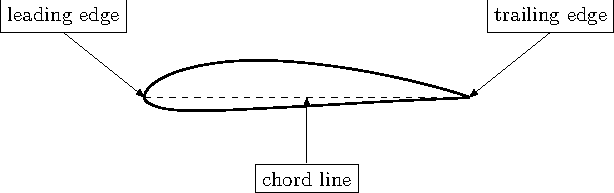
\includegraphics[width=0.5\textwidth]{figures/airfoil}
			\label{fig:airfoil}
		\end{wrapfigure}
		\tableofcontents

	\end{frame}
	
	\begin{frame}{Introduction}
		\section{Introduction}
		The aim of this project is to evaluate the polar curve of the NACA 4415 airfoil (figure \ref{fig:airfoil}) by the validation of a CFD model. 
		
		\begin{figure}[H]
			\centering
			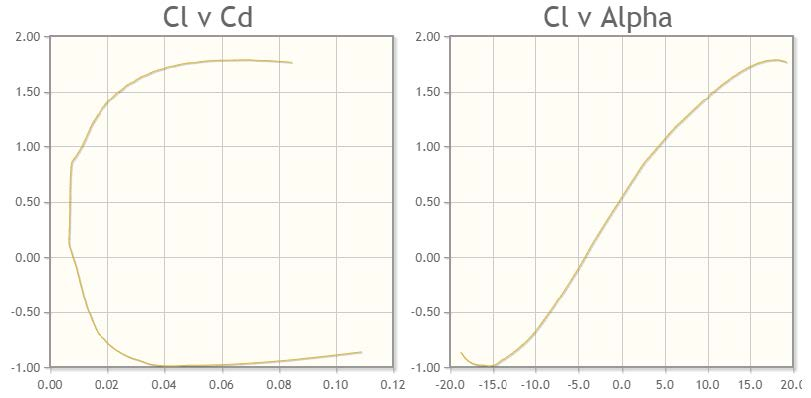
\includegraphics[width=0.4\linewidth]{figures/Lab_ASSIGNMENT}
			\label{fig:labassignment}
		\end{figure}
		
		
		This particular representation permit to individuate, by the tangent curve for the origin, the best attack angle to optimize the working airfoil.
		
		In this point, the maximum $\dfrac{C_L}{C_D}$ permits to have the maximum lift over the minimum drag.
		
		
		
	\end{frame}
	
%	\begin{frame}
%		In this work we provide to:
%		\begin{enumerate}
%			\ra{1.5}
%			\item Draw a geometry that helps to evaluate the project;
%			\item Validate the CFD model by choosing the better combination of parameters like mesh size, URF, scheme and models;
%			\item Evaluate the transient model by the correct choose of the Courant number and the relative time steps;
%			\item Draw the required curves like in the figure \ref{fig:labassignment}.
%		\end{enumerate}
%	\end{frame}
	
	\begin{frame}{Materials \& Methods: Software \& Hardware}
		\begin{wrapfigure}{r}{0.4\linewidth}
			\centering
			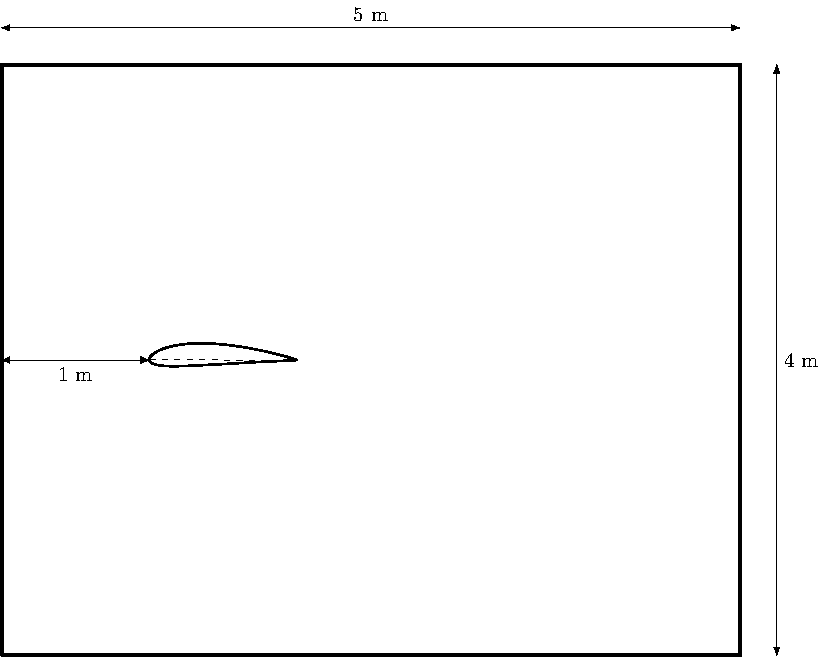
\includegraphics[width=0.5\textwidth]{figures/geometry}
			\label{fig:geometry}
		\end{wrapfigure}
		
		\section{Software \& Hardware}
		\textbf{Software}
		\begin{itemize}
			\item ANSYS 2023 R2 Student version;
			\item Geometry: SpaceClaim
			\item Calculus: Fluent
		\end{itemize}
		\textbf{Hardware}
		\begin{itemize}
			\item CPU: AMD FX 8150 8-core processor 
			\item GPU: ASUS NVidia GeForce GTX 1660 Ti
			\item RAM: 16 GB
		\end{itemize}
		\textbf{Initial Data}:
		\begin{itemize}
			\item Airfoil geometry;
			\item $Re = 1 \times 10^6$, $\rho = \SI{1.225}{\kilogram\per\cubic\meter}$, $\mu = \SI{1.7894e-5}{\kilogram\per\meter\per\second}$, $L = \SI{1}{\meter}$, $\Rightarrow$ \alert{$u = \SI{14.607}{\meter\per\second}$}
		\end{itemize}
		
	\end{frame}
	
	\begin{frame}[shrink=55]{Materials \& Methods: Models \& Scheme}
		\section{Models \& Scheme}
		\begin{landscape}
			\begin{table}[H]
				\ra{1.5}
				\centering
				\begin{tabular}{|cccccccccccc|}
					\hline
					\multicolumn{12}{|c|}{\textbf{Brief Analysis - Hypothetical value of mesh size for testing  model and method (default setting for free steam mesh)}}                                                                                                                                                                                                                                                                                                                                                                                        \\ \hline
					\multicolumn{1}{|c|}{Edge sizing}               & \multicolumn{1}{c|}{Mesh size}              & \multicolumn{1}{c|}{Max Skewness}           & \multicolumn{1}{c|}{\%Skw}                  & \multicolumn{1}{c|}{State}                     & \multicolumn{1}{c|}{Model}                                                                & \multicolumn{1}{c|}{$y^+$}                 & \multicolumn{1}{c|}{Method}                          & \multicolumn{1}{c|}{Iterations} & \multicolumn{1}{c|}{$C_L$}      & \multicolumn{1}{c|}{$\Delta$}    & err\%                               \\ \hline
					\multicolumn{1}{|c|}{}                          & \multicolumn{1}{c|}{}                       & \multicolumn{1}{c|}{}                       & \multicolumn{1}{c|}{}                       & \multicolumn{1}{c|}{}                          & \multicolumn{1}{c|}{\cellcolor[HTML]{96FFFB}}                                             & \multicolumn{1}{c|}{}                      & \multicolumn{1}{c|}{\cellcolor[HTML]{FFCE93}SIMPLE}  & \multicolumn{1}{c|}{1068}       & \multicolumn{1}{c|}{0.39835492} & \multicolumn{1}{c|}{0.015300708} & 3.698899994                         \\ \cline{8-12} 
					\multicolumn{1}{|c|}{}                          & \multicolumn{1}{c|}{}                       & \multicolumn{1}{c|}{}                       & \multicolumn{1}{c|}{}                       & \multicolumn{1}{c|}{}                          & \multicolumn{1}{c|}{\cellcolor[HTML]{96FFFB}}                                             & \multicolumn{1}{c|}{}                      & \multicolumn{1}{c|}{\cellcolor[HTML]{FE996B}SIMPLEC} & \multicolumn{1}{c|}{1737}       & \multicolumn{1}{c|}{0.36678985} & \multicolumn{1}{c|}{0.046865778} & 11.32966043                         \\ \cline{8-12} 
					\multicolumn{1}{|c|}{}                          & \multicolumn{1}{c|}{}                       & \multicolumn{1}{c|}{}                       & \multicolumn{1}{c|}{}                       & \multicolumn{1}{c|}{}                          & \multicolumn{1}{c|}{\cellcolor[HTML]{96FFFB}}                                             & \multicolumn{1}{c|}{}                      & \multicolumn{1}{c|}{\cellcolor[HTML]{F56B00}PISO}    & \multicolumn{1}{c|}{1055}       & \multicolumn{1}{c|}{0.39921114} & \multicolumn{1}{c|}{0.014444488} & \cellcolor[HTML]{34FF34}3.491911393 \\ \cline{8-12} 
					\multicolumn{1}{|c|}{\multirow{-4}{*}{0.00012}} & \multicolumn{1}{c|}{}                       & \multicolumn{1}{c|}{\multirow{-4}{*}{0.75}} & \multicolumn{1}{c|}{\multirow{-4}{*}{0.15}} & \multicolumn{1}{c|}{}                          & \multicolumn{1}{c|}{\multirow{-4}{*}{\cellcolor[HTML]{96FFFB}Viscous $k\omega$ SST}}      & \multicolumn{1}{c|}{\multirow{-4}{*}{5}}   & \multicolumn{1}{c|}{\cellcolor[HTML]{CE6301}Coupled} & \multicolumn{1}{c|}{79}         & \multicolumn{1}{c|}{0.34955502} & \multicolumn{1}{c|}{0.064100608} & 15.49612858                         \\ \cline{1-1} \cline{3-4} \cline{6-12} 
					\multicolumn{1}{|c|}{}                          & \multicolumn{1}{c|}{}                       & \multicolumn{1}{c|}{}                       & \multicolumn{1}{c|}{}                       & \multicolumn{1}{c|}{}                          & \multicolumn{1}{c|}{\cellcolor[HTML]{38FFF8}}                                             & \multicolumn{1}{c|}{}                      & \multicolumn{1}{c|}{\cellcolor[HTML]{FFCE93}SIMPLE}  & \multicolumn{1}{c|}{439}        & \multicolumn{1}{c|}{0.34748226} & \multicolumn{1}{c|}{0.066173368} & 15.99721206                         \\ \cline{8-12} 
					\multicolumn{1}{|c|}{}                          & \multicolumn{1}{c|}{}                       & \multicolumn{1}{c|}{}                       & \multicolumn{1}{c|}{}                       & \multicolumn{1}{c|}{}                          & \multicolumn{1}{c|}{\cellcolor[HTML]{38FFF8}}                                             & \multicolumn{1}{c|}{}                      & \multicolumn{1}{c|}{\cellcolor[HTML]{FE996B}SIMPLEC} & \multicolumn{1}{c|}{610}        & \multicolumn{1}{c|}{0.35107735} & \multicolumn{1}{c|}{0.062578278} & \cellcolor[HTML]{67FD9A}15.1281099  \\ \cline{8-12} 
					\multicolumn{1}{|c|}{}                          & \multicolumn{1}{c|}{}                       & \multicolumn{1}{c|}{}                       & \multicolumn{1}{c|}{}                       & \multicolumn{1}{c|}{}                          & \multicolumn{1}{c|}{\cellcolor[HTML]{38FFF8}}                                             & \multicolumn{1}{c|}{}                      & \multicolumn{1}{c|}{\cellcolor[HTML]{F56B00}PISO}    & \multicolumn{1}{c|}{438}        & \multicolumn{1}{c|}{0.34744313} & \multicolumn{1}{c|}{0.066212498} & 16.00667162                         \\ \cline{8-12} 
					\multicolumn{1}{|c|}{\multirow{-4}{*}{0.00381}} & \multicolumn{1}{c|}{}                       & \multicolumn{1}{c|}{\multirow{-4}{*}{0.7}}  & \multicolumn{1}{c|}{\multirow{-4}{*}{0.04}} & \multicolumn{1}{c|}{}                          & \multicolumn{1}{c|}{\multirow{-4}{*}{\cellcolor[HTML]{38FFF8}Viscous $k\varepsilon$ sdt}} & \multicolumn{1}{c|}{\multirow{-4}{*}{165}} & \multicolumn{1}{c|}{\cellcolor[HTML]{CE6301}Coupled} & \multicolumn{1}{c|}{70}         & \multicolumn{1}{c|}{0.35038373} & \multicolumn{1}{c|}{0.063271898} & 15.29579044                         \\ \cline{1-1} \cline{3-4} \cline{6-12} 
					\multicolumn{1}{|c|}{}                          & \multicolumn{1}{c|}{}                       & \multicolumn{1}{c|}{}                       & \multicolumn{1}{c|}{}                       & \multicolumn{1}{c|}{}                          & \multicolumn{1}{c|}{\cellcolor[HTML]{68CBD0}}                                             & \multicolumn{1}{c|}{}                      & \multicolumn{1}{c|}{\cellcolor[HTML]{FFCE93}SIMPLE}  & \multicolumn{1}{c|}{745}        & \multicolumn{1}{c|}{0.3298986}  & \multicolumn{1}{c|}{0.083757028} & \cellcolor[HTML]{9AFF99}20.24800881 \\ \cline{8-12} 
					\multicolumn{1}{|c|}{}                          & \multicolumn{1}{c|}{}                       & \multicolumn{1}{c|}{}                       & \multicolumn{1}{c|}{}                       & \multicolumn{1}{c|}{}                          & \multicolumn{1}{c|}{\cellcolor[HTML]{68CBD0}}                                             & \multicolumn{1}{c|}{}                      & \multicolumn{1}{c|}{\cellcolor[HTML]{FE996B}SIMPLEC} & \multicolumn{1}{c|}{854}        & \multicolumn{1}{c|}{0.32843196} & \multicolumn{1}{c|}{0.085223668} & 20.6025646                          \\ \cline{8-12} 
					\multicolumn{1}{|c|}{}                          & \multicolumn{1}{c|}{}                       & \multicolumn{1}{c|}{}                       & \multicolumn{1}{c|}{}                       & \multicolumn{1}{c|}{}                          & \multicolumn{1}{c|}{\cellcolor[HTML]{68CBD0}}                                             & \multicolumn{1}{c|}{}                      & \multicolumn{1}{c|}{\cellcolor[HTML]{F56B00}PISO}    & \multicolumn{1}{c|}{565}        & \multicolumn{1}{c|}{0.3297579}  & \multicolumn{1}{c|}{0.083897728} & 20.28202261                         \\ \cline{8-12} 
					\multicolumn{1}{|c|}{\multirow{-4}{*}{0.00265}} & \multicolumn{1}{c|}{\multirow{-12}{*}{0.3}} & \multicolumn{1}{c|}{\multirow{-4}{*}{0.62}} & \multicolumn{1}{c|}{\multirow{-4}{*}{0.11}} & \multicolumn{1}{c|}{\multirow{-12}{*}{Steady}} & \multicolumn{1}{c|}{\multirow{-4}{*}{\cellcolor[HTML]{68CBD0}Spallart - Allmaras VB}}     & \multicolumn{1}{c|}{\multirow{-4}{*}{115}} & \multicolumn{1}{c|}{\cellcolor[HTML]{CE6301}Coupled} & \multicolumn{1}{c|}{65}         & \multicolumn{1}{c|}{0.32774016} & \multicolumn{1}{c|}{0.085915468} & 20.76980517                         \\ \hline
				\end{tabular}
			\end{table}
		\end{landscape}
		\vspace{0.5cm}
		By evaluating the flow impacting the airfoil at $0^\circ$, we can choose the best model/method coupling. \newline
		
		Viscous k$\omega$ SST model with the PISO method seems to be the best coupling at all. \newline
		
		Knowing that PISO make an extra pressure correction step, for the steady state simulation is maybe quite a waste, by the way, knowing also that in this simulation will be a transient case from -8$^\circ$ to -16$^\circ$ and from 8$^\circ$ to 16 $^\circ$, adding ab extra correction step lead maybe to a more accurate results.  
		
		Nevertheless, its preferable working with the same method for all the cases. \newline
		
		
		
		
		
	\end{frame}
	\begin{frame}[shrink=35]{Grid Sensitivity Analysis}
		
	\section{Grid Sensitivity Analysis}
	
	An analysis regarding the sensitivity of the grid will now be provided, starting from a coarse mesh using the methods and parameters just now studied.
	
		\begin{table}[H]
			\centering
			\begin{tabular}{|cccccc|}
				\hline
				\multicolumn{6}{|c|}{\textbf{Mesh   Sensitivity Analysis RF = 0.57}}                                                                                                                                                                                                                    \\ \hline
				\multicolumn{1}{|c|}{Mesh size}                        & \multicolumn{1}{c|}{$C_L$}                            & \multicolumn{1}{c|}{$\Delta$}                        & \multicolumn{1}{c|}{Iter}                         & \multicolumn{1}{c|}{Max Skw}                       & \%Skw \\ \hline
				\multicolumn{1}{|c|}{1.6}                              & \multicolumn{1}{c|}{0.392276}                         & \multicolumn{1}{c|}{}                                 & \multicolumn{1}{c|}{1165}                         & \multicolumn{1}{c|}{0.75}                          & 0.16  \\ \hline
				\multicolumn{1}{|c|}{0.912}                            & \multicolumn{1}{c|}{0.399265}                         & \multicolumn{1}{c|}{0.006989}                         & \multicolumn{1}{c|}{1060}                         & \multicolumn{1}{c|}{0.748}                         & 0.18  \\ \hline
				\multicolumn{1}{|c|}{0.51984}                          & \multicolumn{1}{c|}{0.40253}                          & \multicolumn{1}{c|}{0.003265}                         & \multicolumn{1}{c|}{1019}                         & \multicolumn{1}{c|}{0.733}                         & 0.25  \\ \hline
				\multicolumn{1}{|c|}{0.296309}                         & \multicolumn{1}{c|}{0.402525}                         & \multicolumn{1}{c|}{4.62E-06}                         & \multicolumn{1}{c|}{1052}                         & \multicolumn{1}{c|}{0.771}                         & 0.1   \\ \hline
				\multicolumn{1}{|c|}{0.168896}                         & \multicolumn{1}{c|}{0.401451}                         & \multicolumn{1}{c|}{0.001074}                         & \multicolumn{1}{c|}{1048}                         & \multicolumn{1}{c|}{0.76}                          & 0.13  \\ \hline
				\rowcolor[HTML]{F8FF00} 
				\multicolumn{1}{|c|}{\cellcolor[HTML]{F8FF00}0.096271} & \multicolumn{1}{c|}{\cellcolor[HTML]{F8FF00}0.393783} & \multicolumn{1}{c|}{\cellcolor[HTML]{F8FF00}0.007668} & \multicolumn{1}{c|}{\cellcolor[HTML]{F8FF00}1163} & \multicolumn{1}{c|}{\cellcolor[HTML]{F8FF00}0.772} & 0.1   \\ \hline
				\multicolumn{1}{|c|}{0.054874}                         & \multicolumn{1}{c|}{0.369932}                         & \multicolumn{1}{c|}{0.023851}                         & \multicolumn{1}{c|}{1762}                         & \multicolumn{1}{c|}{0.739}                         & 0.21  \\ \hline
				\multicolumn{1}{|c|}{0.031278}                         & \multicolumn{1}{c|}{0.384137}                         & \multicolumn{1}{c|}{0.014204}                         & \multicolumn{1}{c|}{1428}                         & \multicolumn{1}{c|}{0.751}                         & 0.14  \\ \hline
			\end{tabular}
		\end{table}
		
\begin{figure}[H]
	\centering
	\includegraphics[width=0.5\linewidth]{"figures/mesh analysis"}
	\label{fig:mesh-analysis}
\end{figure}

	\end{frame}
	\begin{frame}[shrink=22]
					\begin{columns}[T] 
	
			\column{0.5\textwidth} 	
These are so the chosen parameters:
		\begin{table}[H]
			\centering
			\begin{tabular}{|c|c|}
				\hline
				Model     & Viscous k$\omega$ SST \\ \hline
				Method    & PISO                  \\ \hline
				Edge Size & 0.00012               \\ \hline
				Mesh size & 0.09627               \\ \hline
			\end{tabular}
		\end{table}
		
		That leads to this mesh:
		\begin{figure}[H]
			\centering
			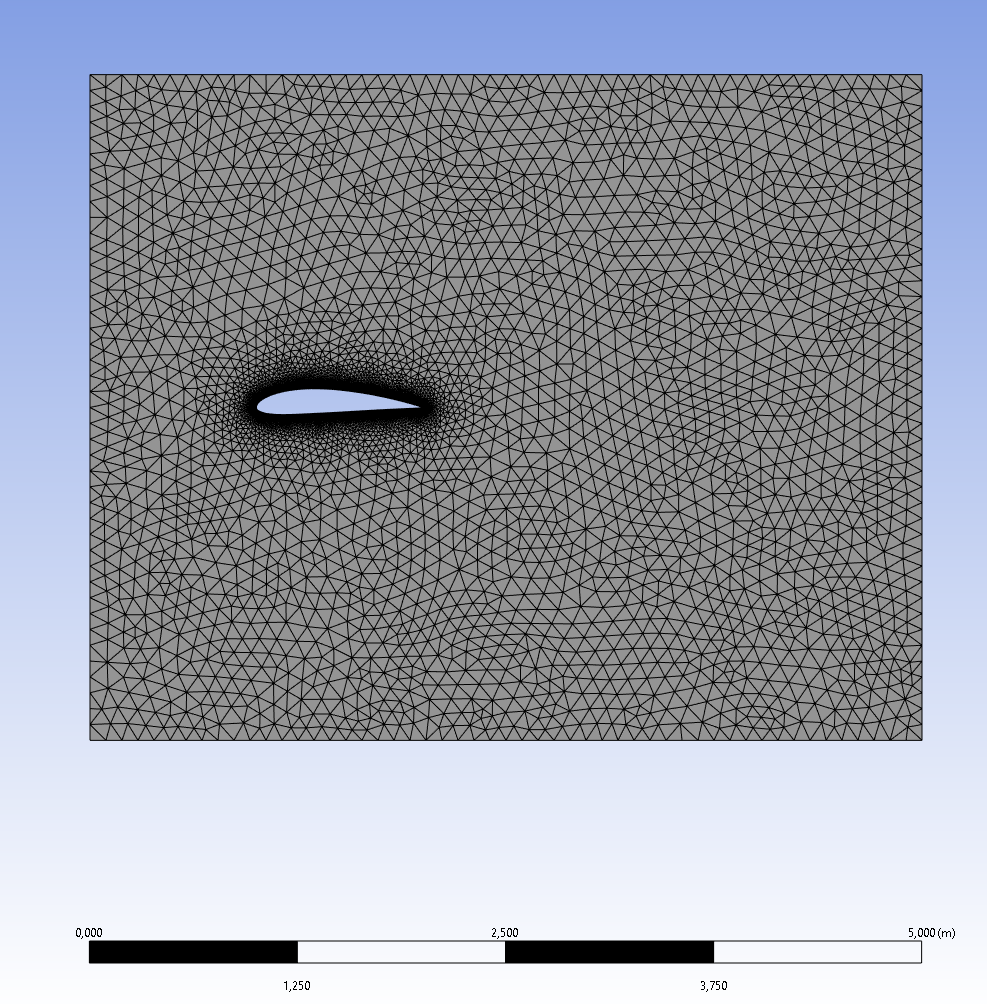
\includegraphics[width=1\linewidth]{figures/mesh}
			\label{fig:mesh}
		\end{figure}
		
		
		\column{0.5\textwidth} 	
		
		With these general conditions, on the boundaries:
		\begin{itemize}
			\item \textbf{Inlet}: velocity inlet type;
			\item \textbf{Outlet}: pressure outlet type;
			\item \textbf{Symmetry}: applied on the top and the bottom of the bounding box;
			\item \textbf{Wall}: on the airfoil edges, no slip conditions are applied.
		\end{itemize}
		
		And on the method:
		\begin{itemize}
			\item \textbf{Skewness Correction} and \textbf{Neighbor Correction} equals to 1;
			\item \textbf{Gradient}: leas squares cell cased
			\item \textbf{Pressure}: second order
			\item \textbf{Momentum}: second order upwind
			\item \textbf{Turbolent Kinetic Energy}: second order upwind
			\item \textbf{Specific Dissipation Rate}: second order upwind
		\end{itemize}
	\end{columns}	
	\end{frame}
	
	\begin{frame}[shrink=55]{Under Relaxation Factors}
		\section{Under Relaxation Factors}
		
	\begin{columns}[T] 
	
	\column{0.5\textwidth} 			
		\begin{table}[H]
			\ra{1.2}
			\centering
			\begin{tabular}{|ccccc|}
				\hline
				\multicolumn{5}{|c|}{URF choice $0^\circ$}                                                                                                                                                                                \\ \hline
				\multicolumn{1}{|c|}{Iterations}                  & \multicolumn{1}{c|}{Controls}                              & \multicolumn{1}{c|}{$C_L$}        & \multicolumn{1}{c|}{$\Delta C_L$}  & err \%                                \\ \hline
				\multicolumn{1}{|c|}{1163}                        & \multicolumn{1}{c|}{Default}                               & \multicolumn{1}{c|}{0.39378324} & \multicolumn{1}{c|}{0.019872388} & 4.804089841                         \\ \hline
				\multicolumn{1}{|c|}{\cellcolor[HTML]{9AFF99}912} & \multicolumn{1}{c|}{0.4 P}                                 & \multicolumn{1}{c|}{0.41253355} & \multicolumn{1}{c|}{0.001122078} & \cellcolor[HTML]{34FF34}0.271258971 \\ \hline
				\multicolumn{1}{|c|}{\cellcolor[HTML]{34FF34}647} & \multicolumn{1}{c|}{0.5 P}                                 & \multicolumn{1}{c|}{0.42725715} & \multicolumn{1}{c|}{0.013601522} & 3.288126905                         \\ \hline
				\multicolumn{1}{|c|}{\cellcolor[HTML]{67FD9A}902} & \multicolumn{1}{c|}{\cellcolor[HTML]{FCFF2F}0.4 P - 0.5 M} & \multicolumn{1}{c|}{0.41844258} & \multicolumn{1}{c|}{0.004786952} & \cellcolor[HTML]{67FD9A}1.157231203 \\ \hline
				\multicolumn{1}{|c|}{925}                         & \multicolumn{1}{c|}{0.4 P - 0.5 M - 0.6 TKE, SDR}          & \multicolumn{1}{c|}{0.41887024} & \multicolumn{1}{c|}{0.005214612} & \cellcolor[HTML]{9AFF99}1.260616718 \\ \hline
			\end{tabular}
		\end{table}
		

		\begin{table}[H]
			\ra{1.2}
			\centering
\begin{tabular}{|ccccc|lll}
	\cline{1-5}
	\multicolumn{5}{|c|}{URF choice $2^\circ$}                                                                                                                                                                               & \multicolumn{1}{c}{} & \multicolumn{1}{c}{} & \multicolumn{1}{c}{} \\ \cline{1-5}
	\multicolumn{1}{|c|}{Iterations}                  & \multicolumn{1}{c|}{Controls}                              & \multicolumn{1}{c|}{$C_L$}    & \multicolumn{1}{c|}{$\Delta C_L$} & err \%                              &                      &                      &                      \\ \cline{1-5}
	\multicolumn{1}{|c|}{1046}                        & \multicolumn{1}{c|}{Default}                               & \multicolumn{1}{c|}{0.603911} & \multicolumn{1}{c|}{0.020460743}  & 3.27701276                          &                      &                      &                      \\ \cline{1-5}
	\multicolumn{1}{|c|}{\cellcolor[HTML]{9AFF99}974} & \multicolumn{1}{c|}{0.4 P}                                 & \multicolumn{1}{c|}{0.612075} & \multicolumn{1}{c|}{0.012296813}  & 1.969469687                         &                      &                      &                      \\ \cline{1-5}
	\multicolumn{1}{|c|}{\cellcolor[HTML]{34FF34}672} & \multicolumn{1}{c|}{0.5 P}                                 & \multicolumn{1}{c|}{0.631829} & \multicolumn{1}{c|}{0.007457117}  & \cellcolor[HTML]{9AFF99}1.194339207 &                      &                      &                      \\ \cline{1-5}
	\multicolumn{1}{|c|}{979}                         & \multicolumn{1}{c|}{\cellcolor[HTML]{F8FF00}0.4 P - 0.5 M} & \multicolumn{1}{c|}{0.619449} & \multicolumn{1}{c|}{0.004922643}  & \cellcolor[HTML]{67FD9A}0.788415353 &                      &                      &                      \\ \cline{1-5}
	\multicolumn{1}{|c|}{\cellcolor[HTML]{67FD9A}929} & \multicolumn{1}{c|}{0.4 P - 0.5 M - 0.6 TKE, SDR}          & \multicolumn{1}{c|}{0.619589} & \multicolumn{1}{c|}{0.004782993}  & \cellcolor[HTML]{34FF34}0.766048872 &                      &                      &                      \\ \cline{1-5}
\end{tabular}
		\end{table}
		

		\begin{table}[H]
			\ra{1.2}
			\centering
\begin{tabular}{|ccccc|}
	\hline
	\multicolumn{5}{|c|}{URF choice $-2^\circ$}                                                                                                                                                                                \\ \hline
	\multicolumn{1}{|c|}{Iterations}                  & \multicolumn{1}{c|}{Controls}                              & \multicolumn{1}{c|}{$C_L$}      & \multicolumn{1}{c|}{$\Delta C_L$} & err \%                              \\ \hline
	\multicolumn{1}{|c|}{1125}                        & \multicolumn{1}{c|}{Default}                               & \multicolumn{1}{c|}{0.19121338} & \multicolumn{1}{c|}{0.034326}     & 15.21934294                         \\ \hline
	\multicolumn{1}{|c|}{901}                         & \multicolumn{1}{c|}{0.4 P}                                 & \multicolumn{1}{c|}{0.20744404} & \multicolumn{1}{c|}{0.018095}     & 8.022953129                         \\ \hline
	\multicolumn{1}{|c|}{\cellcolor[HTML]{34FF34}621} & \multicolumn{1}{c|}{0.5 P}                                 & \multicolumn{1}{c|}{0.22352259} & \multicolumn{1}{c|}{0.002016}     & \cellcolor[HTML]{34FF34}0.894006224 \\ \hline
	\multicolumn{1}{|c|}{\cellcolor[HTML]{67FD9A}815} & \multicolumn{1}{c|}{\cellcolor[HTML]{FFFF00}0.4 P - 0.5 M} & \multicolumn{1}{c|}{0.21978717} & \multicolumn{1}{c|}{0.005752}     & \cellcolor[HTML]{9AFF99}2.550225898 \\ \hline
	\multicolumn{1}{|c|}{\cellcolor[HTML]{9AFF99}823} & \multicolumn{1}{c|}{0.4 P - 0.5 M - 0.6 TKE, SDR}          & \multicolumn{1}{c|}{0.21987279} & \multicolumn{1}{c|}{0.005666}     & \cellcolor[HTML]{67FD9A}2.512263493 \\ \hline
\end{tabular}
		\end{table}
		
			
			\column{0.3\textwidth} 			
			After providing the grid sensitivity analysis, now will be evaluated the right choice of the URFs by their combination, for providing the most accurate results. \newline 
			
			Are used -2$^\circ$, 0$^\circ$, 2$^\circ$ cases, and their experimental data. \newline 
			
			
			With this analysis make from the study of the behavior of 3 point, emerges that the best URFs choice are the 0.4 on Pressure and 0.5 on Momentum due to a combination of less iterations and minor error from the experimental data: \begin{itemize}
				\item $-2^\circ$: 815 iteration, 2.55\% $C_L$ error;
				\item $0^\circ$: 902 iteration, 1.15\% $C_L$ error;
				\item $2^\circ$:  979 iteration, 0.78\% $C_L$ error.
			\end{itemize}
		
	\end{columns}	
		
		
	\end{frame}
	
	\begin{frame}[shrink = 25]{Transient Analysis}
		\section{Transient Analysis}
		The transient analysis is provided by the choose of the \textit{Courant} number. In the vast majority of cases, it can be assumed equal to 10. 
		
		By the \textit{C} number we may know the necessary time step for the transient simulation. 
		\[C = \dfrac{u\cdot\Delta t}{\Delta x}\]
		In which $u$ is the free flow velocity, $\Delta x$ is the minimum value of mesh elements and the $\Delta t$ is the time step size. 
		
		\[\Delta t = \dfrac{C\cdot \Delta s}{u} = \SI{8e-5}{\second}\]
		
		For evaluating the best number of time steps are token the $-10^\circ$ and $10^\circ$ cases. 

\begin{table}[H]
	\centering
	\begin{tabular}{|ccccccc|}
		\hline
		\multicolumn{7}{|c|}{$10^\circ$}                                                                                                                                                                                                                                                                                    \\ \hline
		\multicolumn{1}{|c|}{N. time step}                 & \multicolumn{1}{c|}{It x time step}       & \multicolumn{1}{c|}{$\Delta t$}                 & \multicolumn{1}{c|}{Flow time [s]} & \multicolumn{1}{c|}{$C_L$}    & \multicolumn{1}{c|}{$\Delta C_L$} & err \%                                                  \\ \hline
		\multicolumn{1}{|c|}{1500}                         & \multicolumn{1}{c|}{}                     & \multicolumn{1}{c|}{}                           & \multicolumn{1}{c|}{1.20E-01}      & \multicolumn{1}{c|}{1.1499}   & \multicolumn{1}{c|}{0.110258}     & 8.749544                                                \\ \cline{1-1} \cline{4-7} 
		\multicolumn{1}{|c|}{\cellcolor[HTML]{FCFF2F}2500} & \multicolumn{1}{c|}{}                     & \multicolumn{1}{c|}{}                           & \multicolumn{1}{c|}{2.00E-01}      & \multicolumn{1}{c|}{1.24766}  & \multicolumn{1}{c|}{0.012498}     & \cellcolor[HTML]{FCFF2F}0.991772                        \\ \cline{1-1} \cline{4-7} 
		\multicolumn{1}{|c|}{3750}                         & \multicolumn{1}{c|}{\multirow{-3}{*}{20}} & \multicolumn{1}{c|}{\multirow{-3}{*}{8.00E-05}} & \multicolumn{1}{c|}{3.00E-01}      & \multicolumn{1}{c|}{1.310601} & \multicolumn{1}{c|}{0.050443}     & 4.002872                                                \\ \hline
		\multicolumn{7}{|c|}{$-10^\circ$}                                                                                                                                                                                                                                                                                   \\ \hline
		\multicolumn{1}{|c|}{1500}                         & \multicolumn{1}{c|}{}                     & \multicolumn{1}{c|}{}                           & \multicolumn{1}{c|}{1.20E-01}      & \multicolumn{1}{c|}{-0.53838} & \multicolumn{1}{c|}{0.063893}     & -10.6088                                                \\ \cline{1-1} \cline{4-7} 
		\multicolumn{1}{|c|}{\cellcolor[HTML]{FFFF00}2500} & \multicolumn{1}{c|}{}                     & \multicolumn{1}{c|}{}                           & \multicolumn{1}{c|}{2.00E-01}      & \multicolumn{1}{c|}{-0.58119} & \multicolumn{1}{c|}{0.021081}     & \cellcolor[HTML]{FCFF2F}{\color[HTML]{333333} -3.50021} \\ \cline{1-1} \cline{4-7} 
		\multicolumn{1}{|c|}{3750}                         & \multicolumn{1}{c|}{\multirow{-3}{*}{20}} & \multicolumn{1}{c|}{\multirow{-3}{*}{8.00E-05}} & \multicolumn{1}{c|}{3.00E-01}      & \multicolumn{1}{c|}{-0.58907} & \multicolumn{1}{c|}{0.0132}       & -2.19179                                                \\ \hline
	\end{tabular}
\end{table}
For the $10^\circ$ case, 2500 time steps lead to a more accurate results, while for the $-10^\circ$ case, same time steps value lead to a not-so-bad results with less computational capacity and time. 
	\end{frame}
	
	\begin{frame}[shrink = 65]{Results: $C_L$ Curve}
			\begin{columns}[T] 
			\column{0.5\textwidth} 			
		\section{Results: Linear zone}
		\begin{table}[H]
			\centering
			\begin{tabular}{|ccccc|}
				\hline
				\multicolumn{5}{|c|}{$C_L~vs~ \alpha$}                                                                                             \\ \hline
				\multicolumn{2}{|c|}{Exp. data}                                & \multicolumn{1}{c|}{} & \multicolumn{2}{c|}{CFD data}            \\ \cline{1-2} \cline{4-5} 
				\multicolumn{1}{|c|}{$\alpha$} & \multicolumn{1}{c|}{$C_L$}    & \multicolumn{1}{c|}{} & \multicolumn{1}{c|}{$\alpha$} & $C_L$    \\ \cline{1-2} \cline{4-5} 
				\multicolumn{1}{|c|}{-8.17377} & \multicolumn{1}{c|}{-0.40285} & \multicolumn{1}{c|}{} & \multicolumn{1}{c|}{-8}       & -0.35806 \\ \cline{1-2} \cline{4-5} 
				\multicolumn{1}{|c|}{-6.14642} & \multicolumn{1}{c|}{-0.1959}  & \multicolumn{1}{c|}{} & \multicolumn{1}{c|}{-6}       & -0.16057 \\ \cline{1-2} \cline{4-5} 
				\multicolumn{1}{|c|}{-4.16734} & \multicolumn{1}{c|}{0.01482}  & \multicolumn{1}{c|}{} & \multicolumn{1}{c|}{-4}       & 0.027939 \\ \cline{1-2} \cline{4-5} 
				\multicolumn{1}{|c|}{-2.18825} & \multicolumn{1}{c|}{0.225539} & \multicolumn{1}{c|}{} & \multicolumn{1}{c|}{-2}       & 0.219787 \\ \cline{1-2} \cline{4-5} 
				\multicolumn{1}{|c|}{-0.01609} & \multicolumn{1}{c|}{0.413656} & \multicolumn{1}{c|}{} & \multicolumn{1}{c|}{0}        & 0.418443 \\ \cline{1-2} \cline{4-5} 
				\multicolumn{1}{|c|}{2.011263} & \multicolumn{1}{c|}{0.624372} & \multicolumn{1}{c|}{} & \multicolumn{1}{c|}{2}        & 0.619449 \\ \cline{1-2} \cline{4-5} 
				\multicolumn{1}{|c|}{4.038616} & \multicolumn{1}{c|}{0.861443} & \multicolumn{1}{c|}{} & \multicolumn{1}{c|}{4}        & 0.821015 \\ \cline{1-2} \cline{4-5} 
				\multicolumn{1}{|c|}{6.21078}  & \multicolumn{1}{c|}{1.011909} & \multicolumn{1}{c|}{} & \multicolumn{1}{c|}{6}        & 1.021107 \\ \cline{1-2} \cline{4-5} 
				\multicolumn{1}{|c|}{8.045052} & \multicolumn{1}{c|}{1.166162} & \multicolumn{1}{c|}{} & \multicolumn{1}{c|}{8}        & 1.220264 \\ \cline{1-2} \cline{4-5} 
			\end{tabular}
		\end{table}
		\begin{figure}[H]
			\centering
			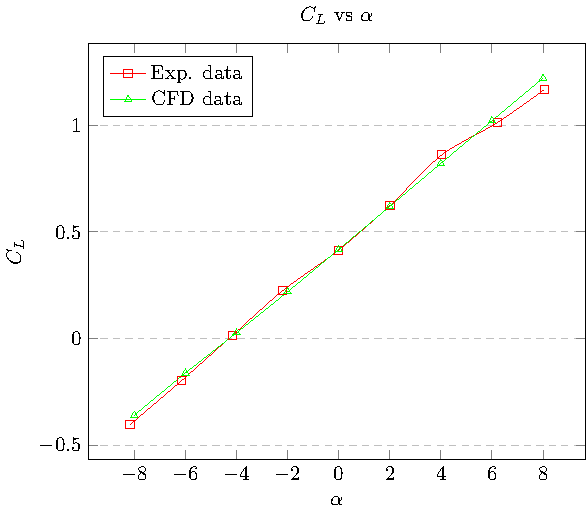
\includegraphics[width=0.8\linewidth]{figures/linear_zone}
			\label{fig:linearzone}
		\end{figure}
		
\column{.01\textwidth}
\rule{.1mm}{2.5\textheight}

			\column{0.5\textwidth} 
		\section{Results: Non-Linear zone}
		\begin{table}[H]
			\centering
			\begin{tabular}{|ccccl|}
				\hline
				\multicolumn{5}{|c|}{$C_L ~ vs~  \alpha$}                                                                                                                           \\ \hline
				\multicolumn{2}{|c|}{Exp. data}                                & \multicolumn{1}{c|}{}          & \multicolumn{2}{c|}{CFD data}                                 \\ \cline{1-2} \cline{4-5} 
				\multicolumn{1}{|c|}{$\alpha$} & \multicolumn{1}{c|}{$C_L$}    & \multicolumn{1}{c|}{}          & \multicolumn{1}{c|}{$\alpha$} & \multicolumn{1}{c|}{$C_L$}    \\ \cline{1-2} \cline{4-5} 
				\multicolumn{1}{|c|}{-16.1384} & \multicolumn{1}{c|}{-0.27057} & \multicolumn{1}{c|}{}          & \multicolumn{1}{c|}{-16}      & -1.0802                       \\ \cline{1-2} \cline{4-5} 
				\multicolumn{1}{|c|}{-14.111}  & \multicolumn{1}{c|}{-0.24435} & \multicolumn{1}{c|}{}          & \multicolumn{1}{c|}{-14}      & -0.89894                      \\ \cline{1-2} \cline{4-5} 
				\multicolumn{1}{|c|}{-12.1319} & \multicolumn{1}{c|}{-0.47037} & \multicolumn{1}{l|}{}          & \multicolumn{1}{c|}{-12}      & -0.72026                      \\ \cline{1-2} \cline{4-5} 
				\multicolumn{1}{|c|}{-10.2494} & \multicolumn{1}{c|}{-0.60227} & \multicolumn{1}{c|}{\textbf{}} & \multicolumn{1}{c|}{-10}      & -0.58119                      \\ \cline{1-2} \cline{4-5} 
				\multicolumn{1}{|c|}{-8.17377} & \multicolumn{1}{c|}{-0.40285} & \multicolumn{1}{c|}{}          & \multicolumn{1}{c|}{-8}       & -0.35806                      \\ \cline{1-2} \cline{4-5} 
				\multicolumn{1}{|c|}{-6.14642} & \multicolumn{1}{c|}{-0.1959}  & \multicolumn{1}{c|}{}          & \multicolumn{1}{c|}{-6}       & -0.16057                      \\ \cline{1-2} \cline{4-5} 
				\multicolumn{1}{|c|}{-4.16734} & \multicolumn{1}{c|}{0.01482}  & \multicolumn{1}{c|}{}          & \multicolumn{1}{c|}{-4}       & 0.027939                      \\ \cline{1-2} \cline{4-5} 
				\multicolumn{1}{|c|}{-2.18825} & \multicolumn{1}{c|}{0.225539} & \multicolumn{1}{c|}{}          & \multicolumn{1}{c|}{-2}       & 0.219787                      \\ \cline{1-2} \cline{4-5} 
				\multicolumn{1}{|c|}{-0.01609} & \multicolumn{1}{c|}{0.413656} & \multicolumn{1}{c|}{}          & \multicolumn{1}{c|}{0}        & \multicolumn{1}{c|}{0.418443} \\ \cline{1-2} \cline{4-5} 
				\multicolumn{1}{|c|}{2.011263} & \multicolumn{1}{c|}{0.624372} & \multicolumn{1}{c|}{}          & \multicolumn{1}{c|}{2}        & 0.619449                      \\ \cline{1-2} \cline{4-5} 
				\multicolumn{1}{|c|}{4.038616} & \multicolumn{1}{c|}{0.861443} & \multicolumn{1}{c|}{}          & \multicolumn{1}{c|}{4}        & 0.821015                      \\ \cline{1-2} \cline{4-5} 
				\multicolumn{1}{|c|}{6.21078}  & \multicolumn{1}{c|}{1.011909} & \multicolumn{1}{c|}{}          & \multicolumn{1}{c|}{6}        & 1.021107                      \\ \cline{1-2} \cline{4-5} 
				\multicolumn{1}{|c|}{8.045052} & \multicolumn{1}{c|}{1.166162} & \multicolumn{1}{c|}{}          & \multicolumn{1}{c|}{8}        & 1.220264                      \\ \cline{1-2} \cline{4-5} 
				\multicolumn{1}{|c|}{10.12068} & \multicolumn{1}{c|}{1.260158} & \multicolumn{1}{c|}{}          & \multicolumn{1}{c|}{10}       & 1.24766                       \\ \cline{1-2} \cline{4-5} 
				\multicolumn{1}{|c|}{12.1963}  & \multicolumn{1}{c|}{1.297678} & \multicolumn{1}{c|}{}          & \multicolumn{1}{c|}{12}       & 1.429237                      \\ \cline{1-2} \cline{4-5} 
				\multicolumn{1}{|c|}{14.27192} & \multicolumn{1}{c|}{1.350259} & \multicolumn{1}{c|}{}          & \multicolumn{1}{c|}{14}       & 1.61119                       \\ \cline{1-2} \cline{4-5} 
				\multicolumn{1}{|c|}{16.10619} & \multicolumn{1}{c|}{1.150596} & \multicolumn{1}{c|}{}          & \multicolumn{1}{c|}{16}       & 1.788569                      \\ \cline{1-2} \cline{4-5} 
			\end{tabular}
		\end{table}
		
		\begin{figure}[H]
			\centering
			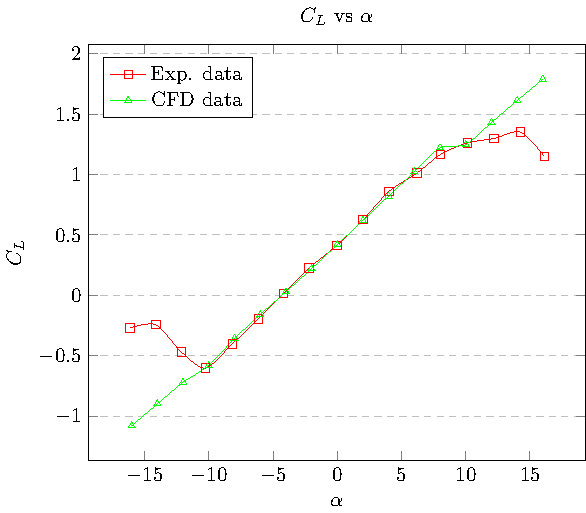
\includegraphics[width=0.8\linewidth]{figures/non-linear_zone}
			\label{fig:non-linearzone}
		\end{figure}	
	\end{columns}	
	\end{frame}
	
	\begin{frame}[shrink = 65]{Results: Polar Curve}	
		\begin{columns}[T] 
			\column{0.5\textwidth} 			
			\begin{table}[H]
				\centering
				\begin{tabular}{|cc|}
					\hline
					\multicolumn{2}{|c|}{$C_L ~vs ~C_D$}      \\ \hline
					\multicolumn{2}{|c|}{CFD data}            \\ \hline
					\multicolumn{1}{|c|}{$C_L$}    & $C_D$    \\ \hline
					\multicolumn{1}{|c|}{-0.35806} & 0.022427 \\ \hline
					\multicolumn{1}{|c|}{-0.16057} & 0.018739 \\ \hline
					\multicolumn{1}{|c|}{0.027939} & 0.01703  \\ \hline
					\multicolumn{1}{|c|}{0.219787} & 0.016623 \\ \hline
					\multicolumn{1}{|c|}{0.418443} & 0.018653 \\ \hline
					\multicolumn{1}{|c|}{0.619449} & 0.022761 \\ \hline
					\multicolumn{1}{|c|}{0.821015} & 0.029031 \\ \hline
					\multicolumn{1}{|c|}{1.021107} & 0.037473 \\ \hline
					\multicolumn{1}{|c|}{1.220264} & 0.048051 \\ \hline
				\end{tabular}
			\end{table}
			
			\begin{figure}[H]
				\centering
				\includegraphics[width=0.8\linewidth]{"figures/plar curve lineartex"}
				\label{fig:plar-curve-lineartex}
			\end{figure}
			
			\column{.01\textwidth}
			\rule{.1mm}{2.5\textheight}
		
			\column{0.5\textwidth} 
			\begin{table}[H]
				\centering
				\begin{tabular}{|ll|}
					\hline
					\multicolumn{2}{|c|}{$C_L ~vs ~C_D$}                        \\ \hline
					\multicolumn{2}{|c|}{CFD data}                              \\ \hline
					\multicolumn{1}{|c|}{$C_L$}    & \multicolumn{1}{c|}{$C_D$} \\ \hline
					\multicolumn{1}{|l|}{-1.0802}  & 0.080922                   \\ \hline
					\multicolumn{1}{|l|}{-0.89894} & 0.059716                   \\ \hline
					\multicolumn{1}{|l|}{-0.72026} & 0.043587                   \\ \hline
					\multicolumn{1}{|l|}{-0.58119} & 0.028905                   \\ \hline
					\multicolumn{1}{|l|}{-0.35806} & 0.022427                   \\ \hline
					\multicolumn{1}{|l|}{-0.16057} & 0.018739                   \\ \hline
					\multicolumn{1}{|l|}{0.027939} & 0.01703                    \\ \hline
					\multicolumn{1}{|l|}{0.219787} & 0.016623                   \\ \hline
					\multicolumn{1}{|c|}{0.418443} & 0.018653                   \\ \hline
					\multicolumn{1}{|l|}{0.619449} & 0.022761                   \\ \hline
					\multicolumn{1}{|l|}{0.821015} & 0.029031                   \\ \hline
					\multicolumn{1}{|l|}{1.021107} & 0.037473                   \\ \hline
					\multicolumn{1}{|l|}{1.220264} & 0.048051                   \\ \hline
					\multicolumn{1}{|l|}{1.24766}  & 0.075529                   \\ \hline
					\multicolumn{1}{|l|}{1.429237} & 0.095512                   \\ \hline
					\multicolumn{1}{|l|}{1.61119}  & 0.11824                    \\ \hline
					\multicolumn{1}{|l|}{1.788569} & 0.143804                   \\ \hline
				\end{tabular}
			\end{table}
			
			\begin{figure}[H]
				\centering
				\includegraphics[width=0.8\linewidth]{"figures/plar curve nnlineartex"}
				\label{fig:plar-curve-nnlineartex}
			\end{figure}						
		\end{columns}
	\end{frame}
	
	\begin{frame}{Conclusions}
		We can see that the CFD model studied provides an excellent approximation for the linear case, from 8$^\circ$ to -8$^\circ$.
		
		By the way, at the externals region of this point, from -10$^\circ$ and 10$^\circ$, the model is absolutely not suitable: the detachment of the fluid vein and the incidences of vorticity do not allow a correct evaluation of this model. 
		\begin{columns}
			\column{0.5\textwidth} 
			\begin{figure}[H]
				\centering
				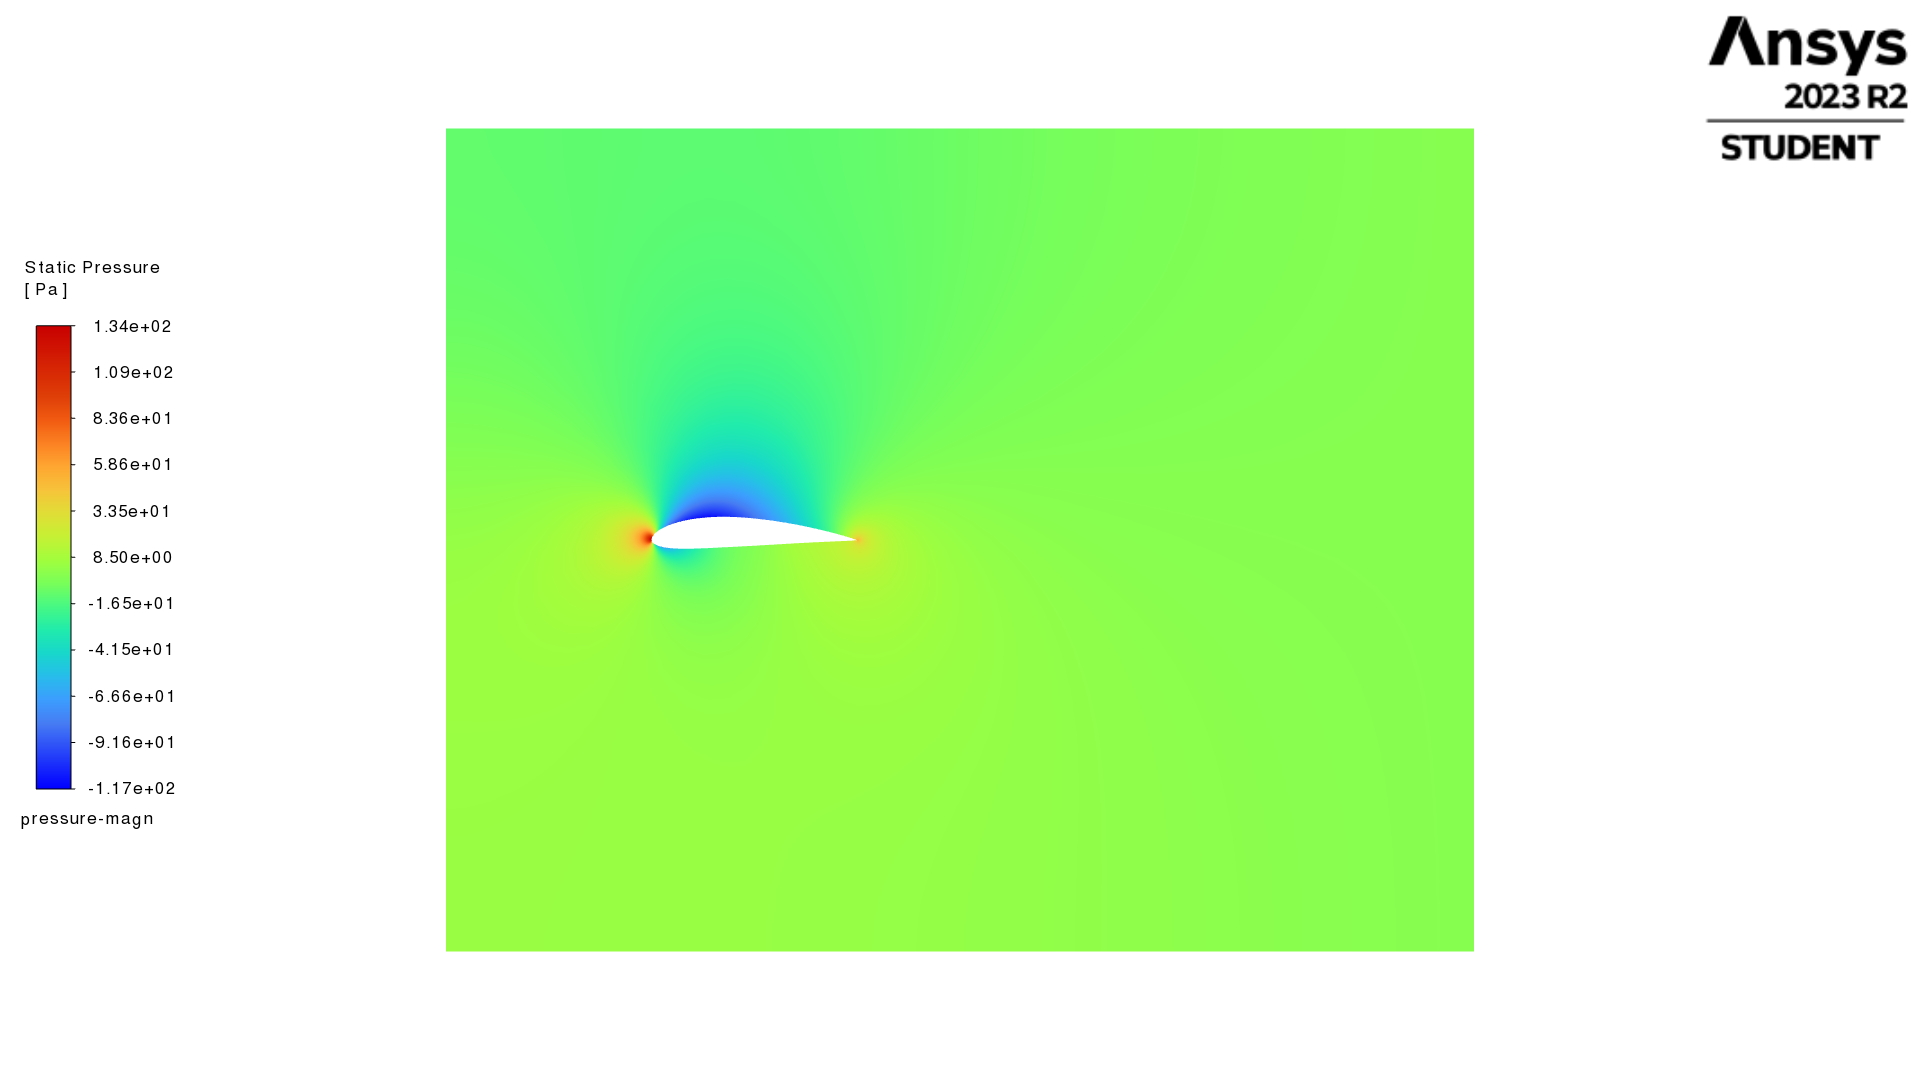
\includegraphics[width=1.1\linewidth]{figures/SYS.1-85-00902}
				\label{fig:sys}
			\end{figure}
			
			\column{0.5\textwidth} 
			\begin{figure}[H]
				\centering
				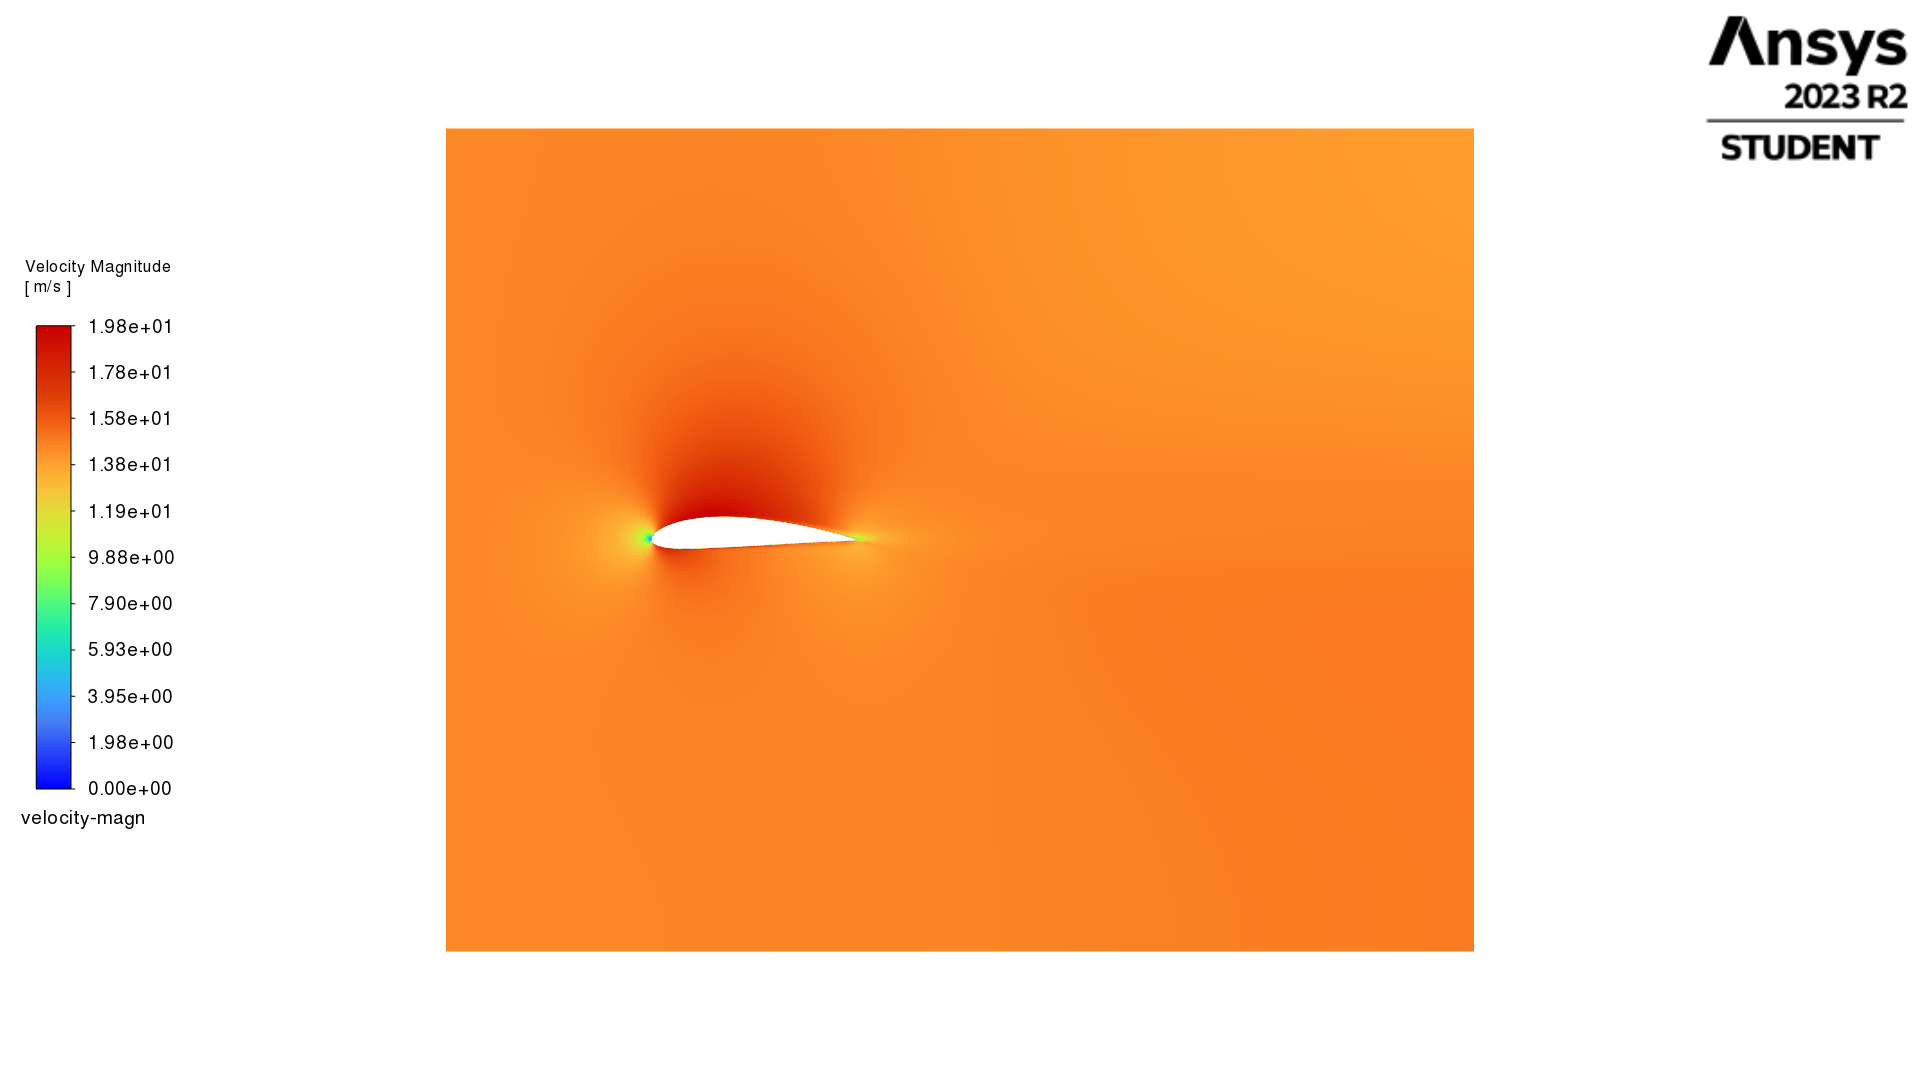
\includegraphics[width=1.1\linewidth]{figures/SYS.1-85-00903}
				\label{fig:sys.2}
			\end{figure}			
		\end{columns}		
	\end{frame}
	
	\begin{frame}
		\begin{figure}[H]
			\centering
			\href{https://youtu.be/w_SOb47J_YI}{
			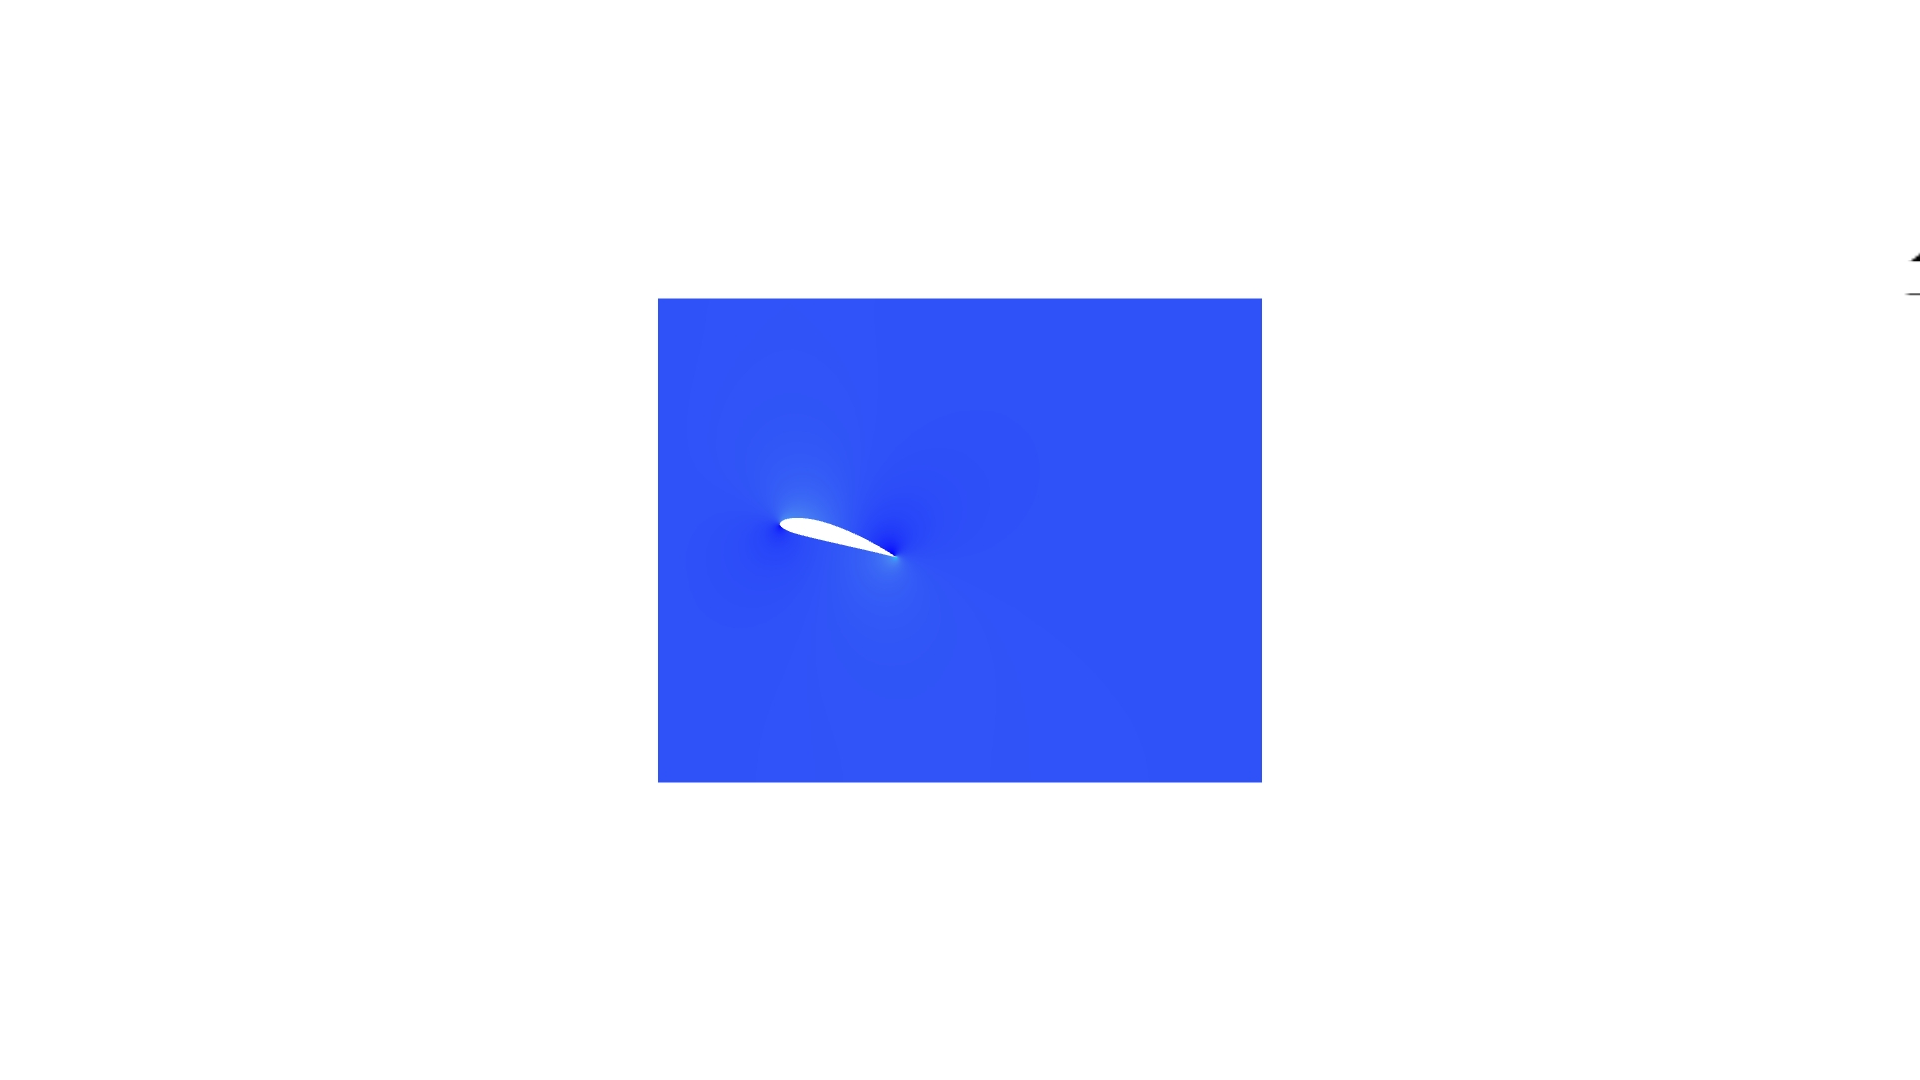
\includegraphics[width=\textheight]{animation-1_1_0000}
			\label{fig:animation-110000}}
		\end{figure}
		
	\end{frame}
	
	
	
	
\end{document}






%\logo{\includegraphics[height=1cm]{overleaf-logo}}